\documentclass[landscape]{article}
\usepackage{geometry}
\usepackage{bookmark}

%\VignetteIndexEntry{Survival Models}
%\VignetteDepends{}
%\VignetteKeywords{Vignettes}

\usepackage{Sweave}
\begin{document}
\Sconcordance{concordance:survivalModels.tex:survivalModels.Rnw:%
1 8 1 1 0 7 1 1 2 1 0 1 1 1 2 5 0 1 1 5 0 1 1 5 0 1 2 5 0 1 2 5 0 1 2 4 %
1 4 0 1 2 2 1 1 2 1 0 1 2 5 0 1 1 5 0 1 1 5 0 1 2 5 0 1 2 5 0 1 2 4 1 4 %
0 1 2 2 1 1 2 1 0 1 2 5 0 1 1 5 0 1 1 5 0 1 2 5 0 1 2 5 0 1 2 4 1 4 0 1 %
2 2 1}


\section{Survival Models}
By overriding the force of mortality and global parameters, we can use makehams to implement a variety of survival models. For instance, it is possible to use a constant force of mortality, $\mu$ or a uniform pdf for $T(x)$.

\subsection{Constant force of mortality}
For CFM, use the \texttt{cfm} function
\begin{Schunk}
\begin{Sinput}
> library(makehams)
> cfm()
> tpx(5,20)
\end{Sinput}
\begin{Soutput}
[1] 0.8187308
\end{Soutput}
\begin{Sinput}
> Ax(20,c=1)
\end{Sinput}
\begin{Soutput}
[1] 0.4505003
\end{Soutput}
\begin{Sinput}
> annx(20,c=1)
\end{Sinput}
\begin{Soutput}
[1] 11.26251
\end{Soutput}
\begin{Sinput}
> Ax(x=21,c=1) - annx(x=21,c=1)*Ax(x=20,c=1)/annx(x=20,c=1)
\end{Sinput}
\begin{Soutput}
[1] -5.551115e-17
\end{Soutput}
\begin{Sinput}
> thV(t=0,h=1,s=0.05)
\end{Sinput}
\begin{Soutput}
[1] 0
\end{Soutput}
\begin{Sinput}
> par(mfrow=c(2,2))
> plot(tpx, 0, 100)
> plot(tqx, 0, 100)
> plot(function(x) sapply(x, function(s) Ax(s,c=1)), 20, 50, ylab="Abarx", xlab="x")
> plot(function(x) sapply(x, function(s) annx(s,c=1)), 20, 50, ylab="abarx", xlab="x")
\end{Sinput}
\end{Schunk}
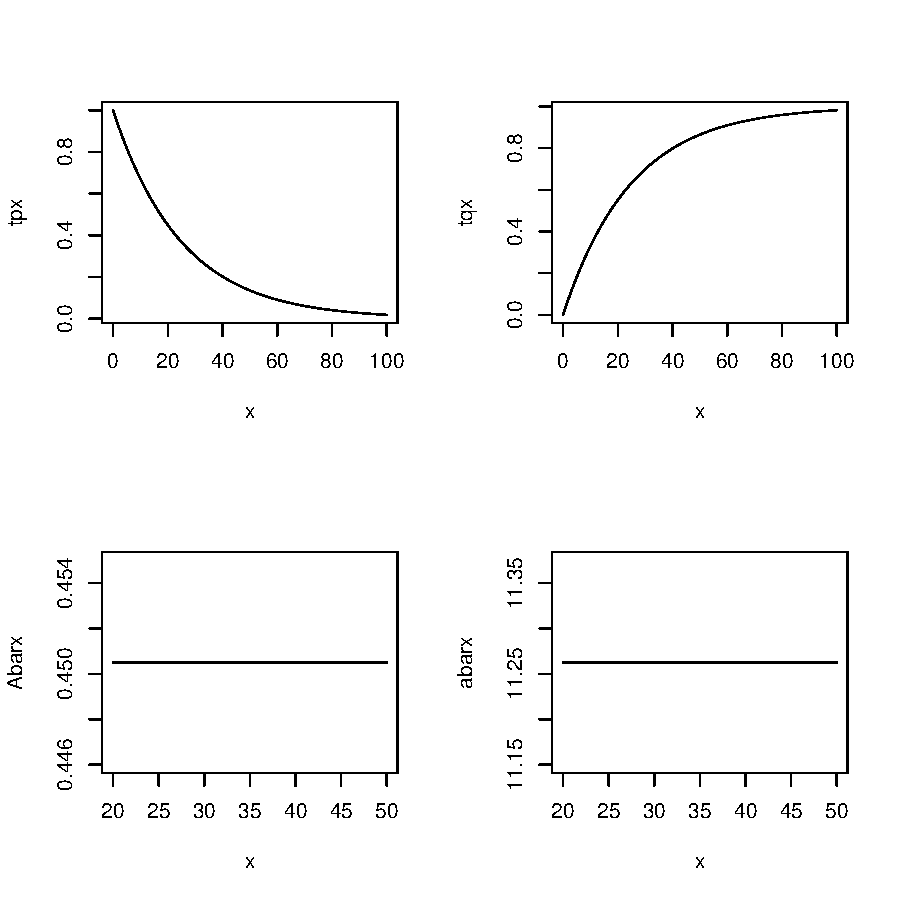
\includegraphics{survivalModels-001}

\subsection{De Moivre's Law}
For De Moivre's Law, we can use the \texttt{demoivres} function
\begin{Schunk}
\begin{Sinput}
> demoivres()
> tpx(5,20)
\end{Sinput}
\begin{Soutput}
[1] 0.9375
\end{Soutput}
\begin{Sinput}
> Ax(x=20,c=1)
\end{Sinput}
\begin{Soutput}
[1] 0.2510299
\end{Soutput}
\begin{Sinput}
> annx(x=20,c=1)
\end{Sinput}
\begin{Soutput}
[1] 15.35084
\end{Soutput}
\begin{Sinput}
> Ax(x=21,c=1) - annx(x=21,c=1)*Ax(x=20,c=1)/annx(x=20,c=1)
\end{Sinput}
\begin{Soutput}
[1] 0.003893153
\end{Soutput}
\begin{Sinput}
> thV(t=0,h=1,s=0.05)
\end{Sinput}
\begin{Soutput}
[1] 0.003891068
\end{Soutput}
\begin{Sinput}
> par(mfrow=c(2,2))
> plot(tpx, 0, 50)
> plot(tqx, 0, 50)
> plot(function(x) sapply(x, function(s) Ax(s,c=1)), 20, 50, ylab="Abarx", xlab="x")
> plot(function(x) sapply(x, function(s) annx(s,c=1)), 20, 50, ylab="abarx", xlab="x")
\end{Sinput}
\end{Schunk}
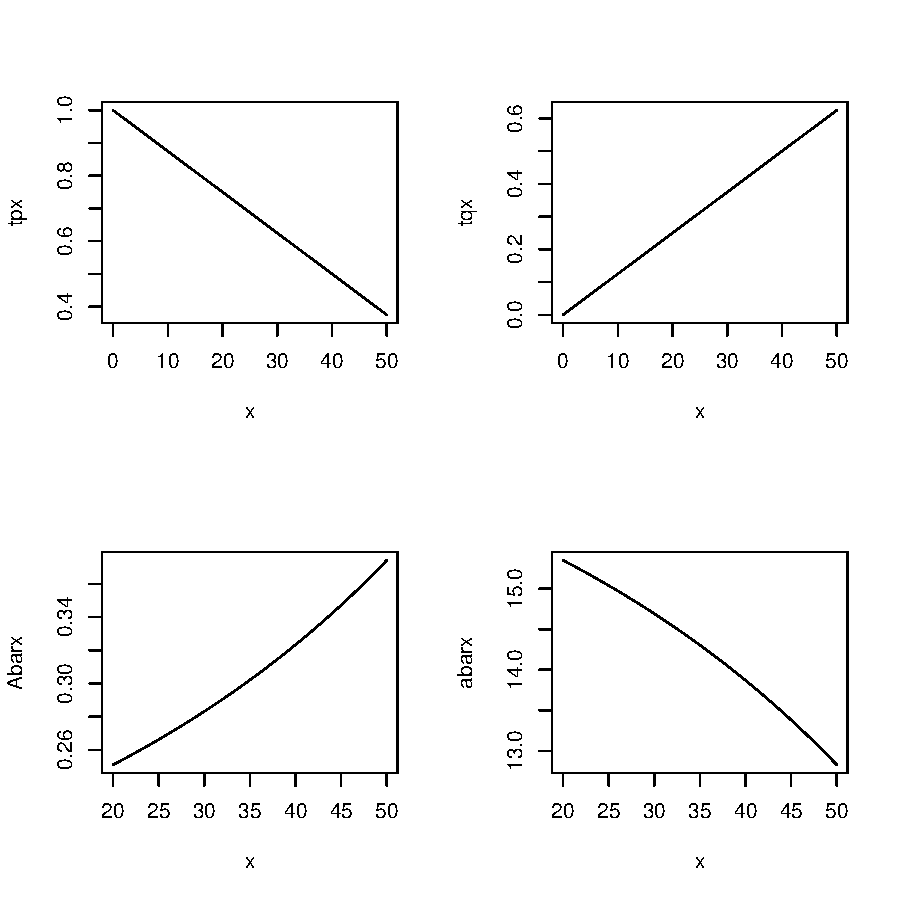
\includegraphics{survivalModels-002}

\subsection{Makeham's Law}
For Makeham's Law, we can use the \texttt{makehams} function
\begin{Schunk}
\begin{Sinput}
> makehams()
> tpx(5,20)
\end{Sinput}
\begin{Soutput}
[1] 0.9987601
\end{Soutput}
\begin{Sinput}
> Ax(x=20,c=1)
\end{Sinput}
\begin{Soutput}
[1] 0.05043333
\end{Soutput}
\begin{Sinput}
> annx(x=20,c=1)
\end{Sinput}
\begin{Soutput}
[1] 19.46226
\end{Soutput}
\begin{Sinput}
> Ax(x=21,c=1) - annx(x=21,c=1)*Ax(x=20,c=1)/annx(x=20,c=1)
\end{Sinput}
\begin{Soutput}
[1] 0.002400081
\end{Soutput}
\begin{Sinput}
> thV(t=0,h=1,s=0.05)
\end{Sinput}
\begin{Soutput}
[1] 0.002434979
\end{Soutput}
\begin{Sinput}
> par(mfrow=c(2,2))
> plot(tpx, 0, 50)
> plot(tqx, 0, 50)
> plot(function(x) sapply(x, function(s) Ax(s,c=1)), 20, 50, ylab="Abarx", xlab="x")
> plot(function(x) sapply(x, function(s) annx(s,c=1)), 20, 50, ylab="abarx", xlab="x")
\end{Sinput}
\end{Schunk}
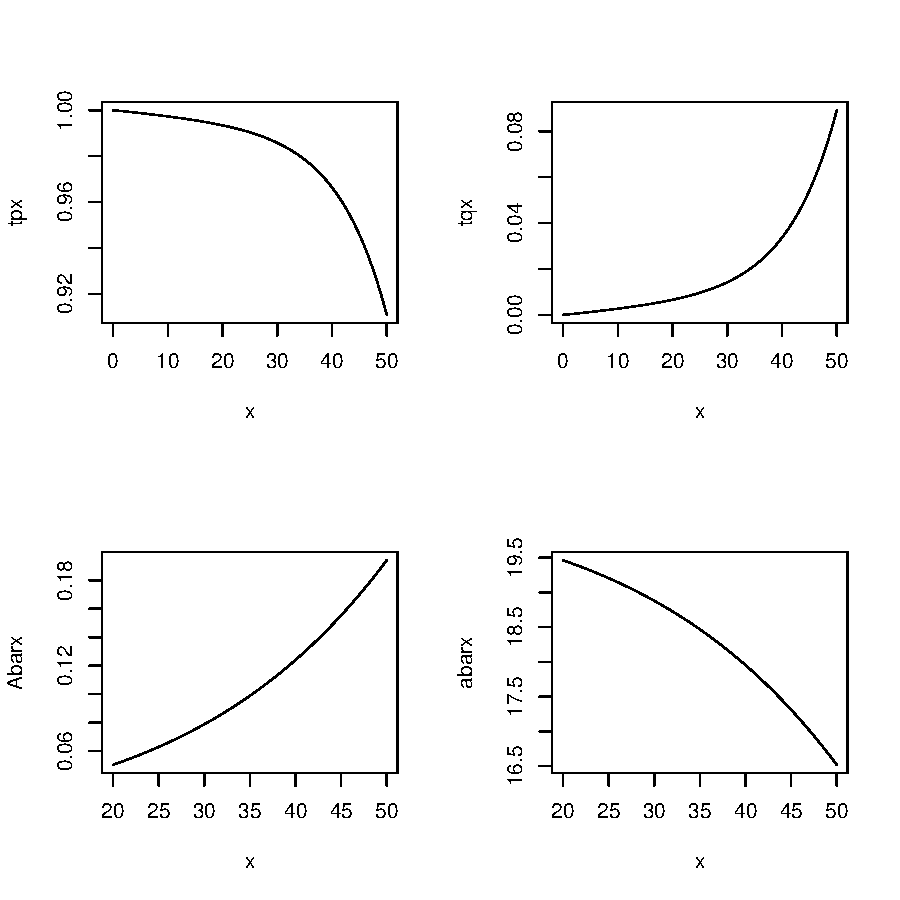
\includegraphics{survivalModels-003}


\end{document}
